% ~1,5 páginas
\section{Resultados preliminares}
\label{sec:resultados}

Todos os valores desta secção vêm das 149 cenas descritas na
\cref{sec:abordagem} e de validação cruzada em cinco partes agrupada por
cena: nenhuma cena contribui ao mesmo tempo para o treino e para o teste.

\subsection{Previsão}

% A tabela, as figuras e os números de classificação saem de
% scripts/make_article_figures.py; os modelos alternativos e a curva de
% aprendizagem, de scripts/compare_alternative_models.py.

\begin{table}[t]
\centering
\caption{Erro final de posição (FDE), em metros: média e desvio-padrão
  das cinco partes da validação cruzada. «(mapa)»: posição prevista
  diretamente em coordenadas do mapa. Os três últimos modelos usam o
  referencial do veículo e a correção à velocidade constante.}
\label{tab:previsao}
\begin{tabular*}{\textwidth}{@{\extracolsep{\fill}}lccc@{}}
\toprule
Modelo & \un{1}{s} & \un{3}{s} & \un{5}{s} \\
\midrule
Velocidade constante & $0,68 \pm 0,02$ & $4,97 \pm 0,35$ & $12,57 \pm 0,90$ \\
Aceleração constante & $0,44 \pm 0,02$ & $3,32 \pm 0,12$ & $9,71 \pm 0,35$ \\
Floresta aleatória (mapa)
  & $0,89 \pm 0,10$ & $4,25 \pm 0,37$ & $10,02 \pm 0,73$ \\
\midrule
Árvore de decisão & $0,43 \pm 0,02$ & $2,78 \pm 0,14$ & $7,50 \pm 0,35$ \\
Floresta aleatória & $0,39 \pm 0,01$ & $2,47 \pm 0,12$ & $6,66 \pm 0,32$ \\
\emph{Gradient boosting} & $0,37 \pm 0,01$ & $2,36 \pm 0,10$ & $6,52 \pm 0,34$ \\
\bottomrule
\end{tabular*}
\end{table}

A \cref{tab:previsao} mostra três coisas. A velocidade constante erra
\un{4,97}{m} a \un{3}{s} e \un{12,57}{m} a \un{5}{s}, valores coerentes
com os \un{5,7}{m} e \un{14,1}{m} publicados para o mesmo conjunto de
dados em horizontes ligeiramente maiores (\cref{tab:baselines}). A
representação conta mais do que o modelo: a mesma floresta aleatória, a
prever a posição em coordenadas do mapa, perde para a aceleração
constante; no referencial do veículo e a prever a correção, reduz o erro
da velocidade constante para cerca de metade a 3 e a \un{5}{s}. E os três modelos clássicos ficam
próximos, com a floresta aleatória e o \emph{gradient boosting}
praticamente empatados.

\begin{figure}[t]
\centering
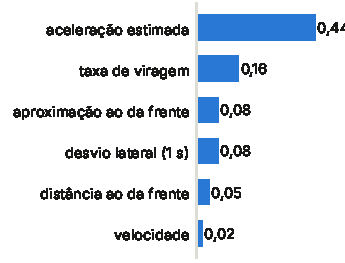
\includegraphics{figuras/importancias.pdf}\hfill
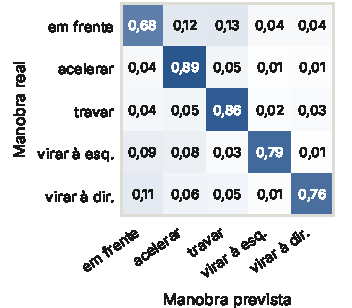
\includegraphics{figuras/confusao.pdf}
\caption{Esquerda: peso das seis variáveis mais importantes na floresta
  aleatória de previsão. Direita: matriz de confusão da floresta
  aleatória na classificação de manobras (cada linha soma 1).}
\label{fig:previsao}
\end{figure}

A \cref{fig:previsao} mostra de onde vem o ganho. As variáveis com mais
peso são a aceleração estimada (0,44), a taxa de viragem (0,16) e a
velocidade de aproximação ao veículo da frente (0,08): o modelo aprende a
prolongar travagens e curvas que já começaram e a contar com quem vai à
frente. Sem as
três variáveis do veículo da frente, o erro a \un{3}{s} sobe de
\un{2,47}{m} para \un{2,68}{m}.

\paragraph{Outros modelos e mais dados.}
Com a mesma representação, a regressão linear erra \un{3,10}{m} a
\un{3}{s}, os vizinhos mais próximos \un{2,70}{m} (\un{3,86}{m} sem
normalizar as variáveis) e uma máquina de vetores de suporte
\un{2,34}{m}, ao nível do \emph{gradient boosting} mas com quase o triplo
do tempo de treino da floresta. As árvores juntam bom resultado, treino
rápido, nenhuma normalização e o peso de cada variável. Treinar com mais cenas quase
não ajuda (\un{2,58}{m} com 25 cenas, \un{2,47}{m} com 119): o próximo
ganho virá de variáveis novas (mapa, semáforos) e não de mais dados do
mesmo tipo.

\paragraph{Segundo conjunto de cenas.}
Para confirmar que o resultado não depende da amostra, repetiu-se a
validação num segundo conjunto, de 178 cenas diferentes (6\,142
amostras), extraído sem as variáveis do veículo da frente. A \un{3}{s},
a velocidade constante erra \un{4,68}{m}, a aceleração constante
\un{3,28}{m}, a floresta em coordenadas do mapa \un{4,03}{m} e a
floresta proposta \un{2,69}{m}. A ordem e as proporções mantêm-se.

\paragraph{Classificação de manobras.}
O mesmo conjunto de variáveis serve para classificar a manobra dos
\un{3}{s} seguintes em cinco classes. Com a mesma validação cruzada, a
floresta aleatória acerta 74,9\% (F1 macro 0,74) e o \emph{gradient
boosting} 79,8\% (0,77); prever sempre a classe mais frequente daria
55\%. A classe mais difícil é «em frente», confundida com acelerações e
travagens ligeiras (\cref{fig:previsao}).

\subsection{Planeamento}

% Os valores da tabela e do texto saem de scripts/evaluate_planner_cv.py.

\begin{table}[t]
\centering
\caption{Planeador A* em 909 situações de 121 cenas, por fonte de
  previsão. Conflito: o plano passa a menos de \un{3,5}{m} da posição
  real de um veículo. Travagens máximas: passos de \un{0,1}{s} com a
  travagem mais forte, em média por situação. Intervalos de confiança a
  95\% por reamostragem das cenas.}
\label{tab:planeamento}
\begin{tabular*}{\textwidth}{@{\extracolsep{\fill}}lccc@{}}
\toprule
Previsão & Conflitos (\%) & Travagens máximas & Velocidade (m/s) \\
\midrule
Nenhuma & 21,8 [16,3; 27,3] & 0,11 & 5,49 \\
Velocidade constante & 20,7 [15,6; 25,7] & 0,02 & 5,38 \\
Floresta aleatória & 20,2 [15,1; 25,4] & 0,02 & 5,36 \\
Futuro real & 16,7 [12,0; 21,4] & 0,04 & 5,37 \\
\bottomrule
\end{tabular*}
\end{table}

A \cref{tab:planeamento} compara as quatro fontes de previsão. Cada
situação é um instante de uma cena com pelo menos um veículo à frente do
veículo autónomo, a menos de \un{25}{m}; em cada parte da validação
cruzada, a floresta é treinada nas outras quatro. Conhecer o futuro é
melhor do que qualquer das outras fontes: menos 3,5 a 5,1 pontos
percentuais de conflitos, com intervalos de confiança que excluem o zero.
Planear sem previsão distingue-se sobretudo pelas travagens máximas,
cinco vezes mais frequentes. Entre a velocidade constante e a floresta
aleatória a diferença é de 0,4 pontos percentuais, com intervalo de
confiança de $-0,8$ a $1,9$: não se distinguem. O ganho de exatidão da
\cref{tab:previsao} não chega, por agora, ao plano, o que está de acordo
com a literatura da \cref{sec:integracao}.

O valor do futuro real mostra onde está o problema: mesmo com previsões
perfeitas há conflitos em 16,7\% das situações, pelo que o limite está no
planeador e na avaliação, e não nas previsões. Há quatro causas
identificadas. O caminho é uma reta na direção atual do veículo, e não a
faixa. As posições dos outros veículos, previstas e reais, são
interpoladas em linha reta entre o instante atual e os \un{3}{s}. O
critério de conflito é uma distância entre centros, que conta veículos da
faixa do lado; em 3,7\% das situações já há um veículo a menos de
\un{3,5}{m} no instante inicial. E o teste executa um único plano de
\un{3}{s} em ciclo aberto, sem voltar a planear.
